\chapter{Neue Fahrzeuge hinzufügen}
\label{cha:newentries}
%
\begin{figure}[htp]
	\centering
	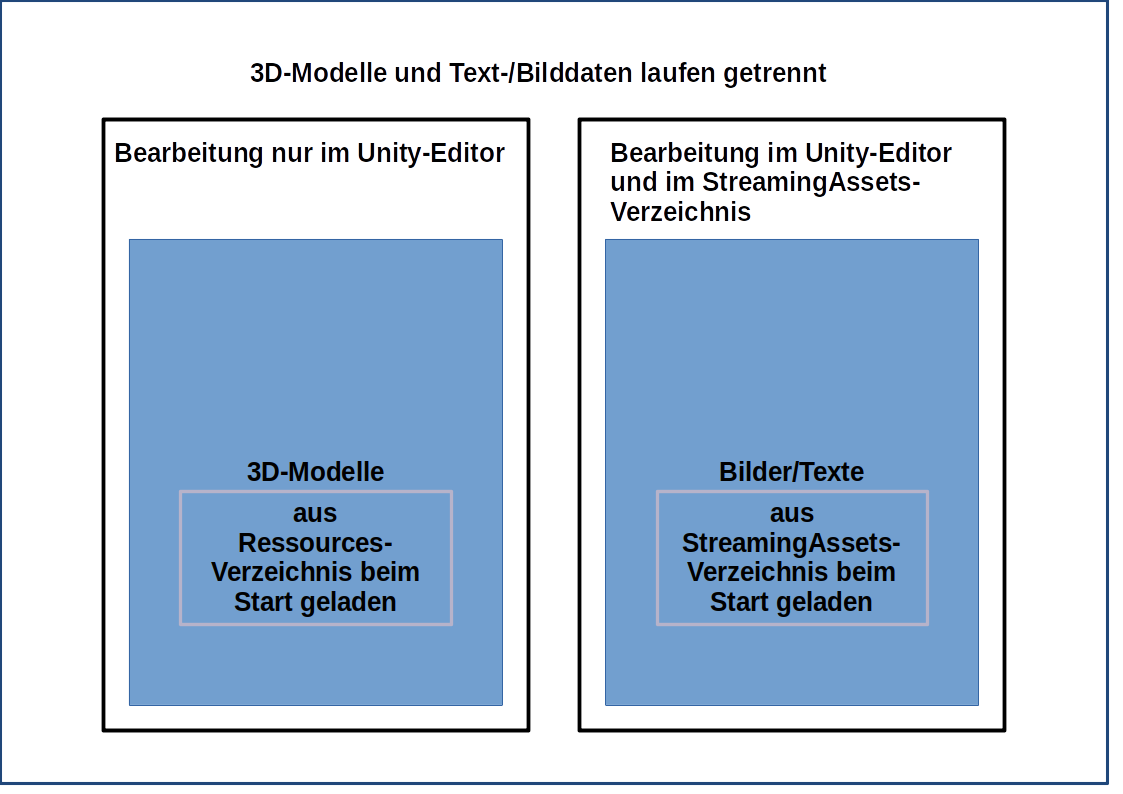
\includegraphics[width=0.8\linewidth]{img/new_entries}
	\caption[structure]{Trennung der Ladevorgänge nach geladenem Inhalt}
	\label{fig:newentry}
\end{figure}
%
\section{Neues Fahrzeug-Model einbauen}
%
\subsection{Import des 3D-Modells}
%
\begin{enumerate}
	\item Model als .fbx Datei per Drag'n'Drop in \enquote{Models}-Verzeichnis im Project-Panel laden
	\item \vhs{} aus Scenes-Verzeichnis per Doppelklick laden
	\item In Punkt 1 importierte .fbx Datei aus Models Verzeichnis per Drag'n'Drop in die Hierarchy ziehen und unter den \enquote{ModelController} einordnen
	\item Im Inspector: Layer auf \enquote{Vehicle} stellen, sonst wird es ausgeblendet
\end{enumerate}
%
\newpage
\subsection{Import der Texturen}
%
\begin{enumerate}
	\item Im Project-Panel im Verzeichnis \enquote{Materials} neuen Ordner erstellen und mit Namen des Fahrzeugs benennen
	\item Bilddateien (.tiff) für BaseColor-, Matelness- und Normal-Kanal in erstelltes Verzeichnis importieren
	\item neues Material erstellen (RMB $\Rightarrow$ Create $\Rightarrow$ Material)
	\item Texturen (.tiff) per Drag'n'Drop ins Project Panel laden und dem zuvor erstellen Material zuweisen
	\item Material(s) dem geladenen 3D-Model zuweisen 
	\item Falls transparente Oberflächen (Glass) benötigt werden:
	\begin{enumerate}
		\item Material kopieren
		\item Im Inspector Surface Type auf Transparent umstellen
		\item Materials mit \enquote{\_transparent} bzw. \enquote{\_opaque} umbenennen
		\item \enquote{\_opaque}-Material dem ersten Material Slot des Modells zuweisen und \enquote{\_transparent}-Material dem zweiten Slot zuweisen
	\end{enumerate}
	\item Model in der Hierarchy auswählen und Rotations und Translations Werte auf 0 setzten
	\item Modell aus Hierarchy per Drag'n'Drop in \path{/Resources/model_prefabs} zur entsprechenden Seite hinzufügen
	\item In Prefab Abfrage \enquote{Original Prefab} auswählen
	\item Prefab mit führender Nummer umbenennen, Nummern sind nach Erscheinungsjahr sortiert
	\item Nach Erstellung des Prefab geladene 3D-Modell wieder aus der Hirarchy löschen (wird später dynamisch geladen)
	\item \pres aus Scenes-Verzeichnis laden
	\item In der Hirarchy \enquote{\_app}-Object auswählen
	\item Im Inspector unter \emph{left-} bzw. \emph{right Vehicles} Size erhöhen und den Namen des neue Fahrzeug-Prefabs aus \path{/Resources/model_prefabs} entsprechend des Erscheinungsjahres eintragen 
\end{enumerate}
%
\newpage
\section{Texte und Bilder hinzufügen}
%
\begin{enumerate}
	\item Im Verzeichnis \path{/StreamingAssets/[Seite]/} ein vorhadenes Verzeichnis duplizieren und entsprechend der zuvor genutzten Prefab Bezeichnung umbennen
	\item unter \path{/Text/} englischen und deutschen Text ersetzen dabei \textbf{Sytanx einhalten!}
	\item unter \path{/Images/} Gallery-Bilder und \emph{titlePic} ersetzen (Nummerierung der Bilder entspricht der Lade-Reihenfolge)
	\item neues \emph{titlePic} rendern mit Hilfe der \enquote{base.blend}-Datei (\path{/blend_files_for_titlePic/scene/base.blend})
	\item Mit \emph{File} $\Rightarrow$ \emph{Append} Modell aus anderer \emph{.blend}-Datei importieren und entsprechend der vorhandenen Fahrzeuge ausrichten
	\item \emph{F12} drücken für Still-Render und über \emph{Image $\Rightarrow$ Save As} als \enquote{titlePic.png} abspeichern
	\item \emph{titlePic.png} mit den Gallery-Bildern unter \path{\Images\} einordnen
	\end{enumerate}
	%